\begin{figure}[H]
    \centering
    \begin{subfigure}{0.8\linewidth}
        \centering
        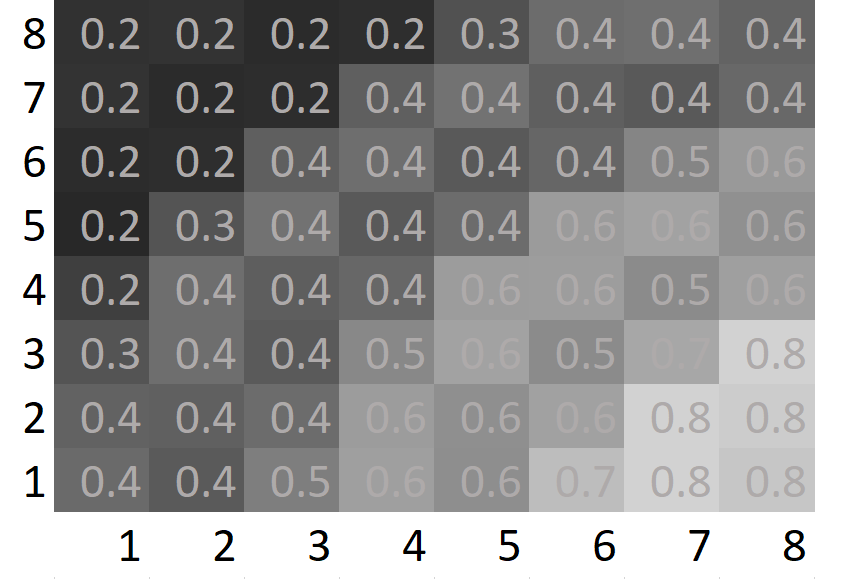
\includegraphics[width=0.45\linewidth]{image/grayscale-explain.png}
    \end{subfigure}
    \caption{ตัวอย่างภาพเฉดเทาที่แสดงระดับความเข้มของภาพในแต่ละระดับ}
    \label{figure:grayscale-explain}
\end{figure}